\documentclass[a4paper,12pt]{article}

\usepackage{other/lab_preamble}

\graphicspath{{data/}}

\begin{document}

\LabTitle{2.3.1}{Получение и измерение вакуума}

\tableofcontents
\listoffigures
\listoftables

\newpage

\textbf{Цель работы}:
\begin{enumerate}
  \item измерение объемов форвакуумной и высоковакуумной частей установки.
  \item определение скорости откачки системы в стационарном режиме, а также по ухудшению и по улучшению вакуума.
\end{enumerate}

\textbf{Приборы}:
\begin{enumerate}
  \item вакуумная установка с манометрами: масляным, термопарным и ионизационным.
\end{enumerate}

\section{Краткая Теория.}

По степени разрежения вакуумные установки принято делить на три класса:
\begin{enumerate}
  \item низковакуумные: до $10^{-2} - 10^{-3}$ торр.
  \item высоковакуумные: до $10^{-4} - 10^{-7}$ торр.
  \item установки сверхвысокого вакуума: до $10^{-8} - 10^{-11}$ торр.
\end{enumerate}
В данной работе изучаются традиционные методы откачки механическим форвакуумным насосом до $10^{-2} \torr$ \\
и диффузионным масляным насосом до $10^{-5} \torr$, а также методы измерения вакуума в этом диапазоне.

\subsection{Экспериментальная установка.}

\begin{figure} [H]
  \begin{center}
    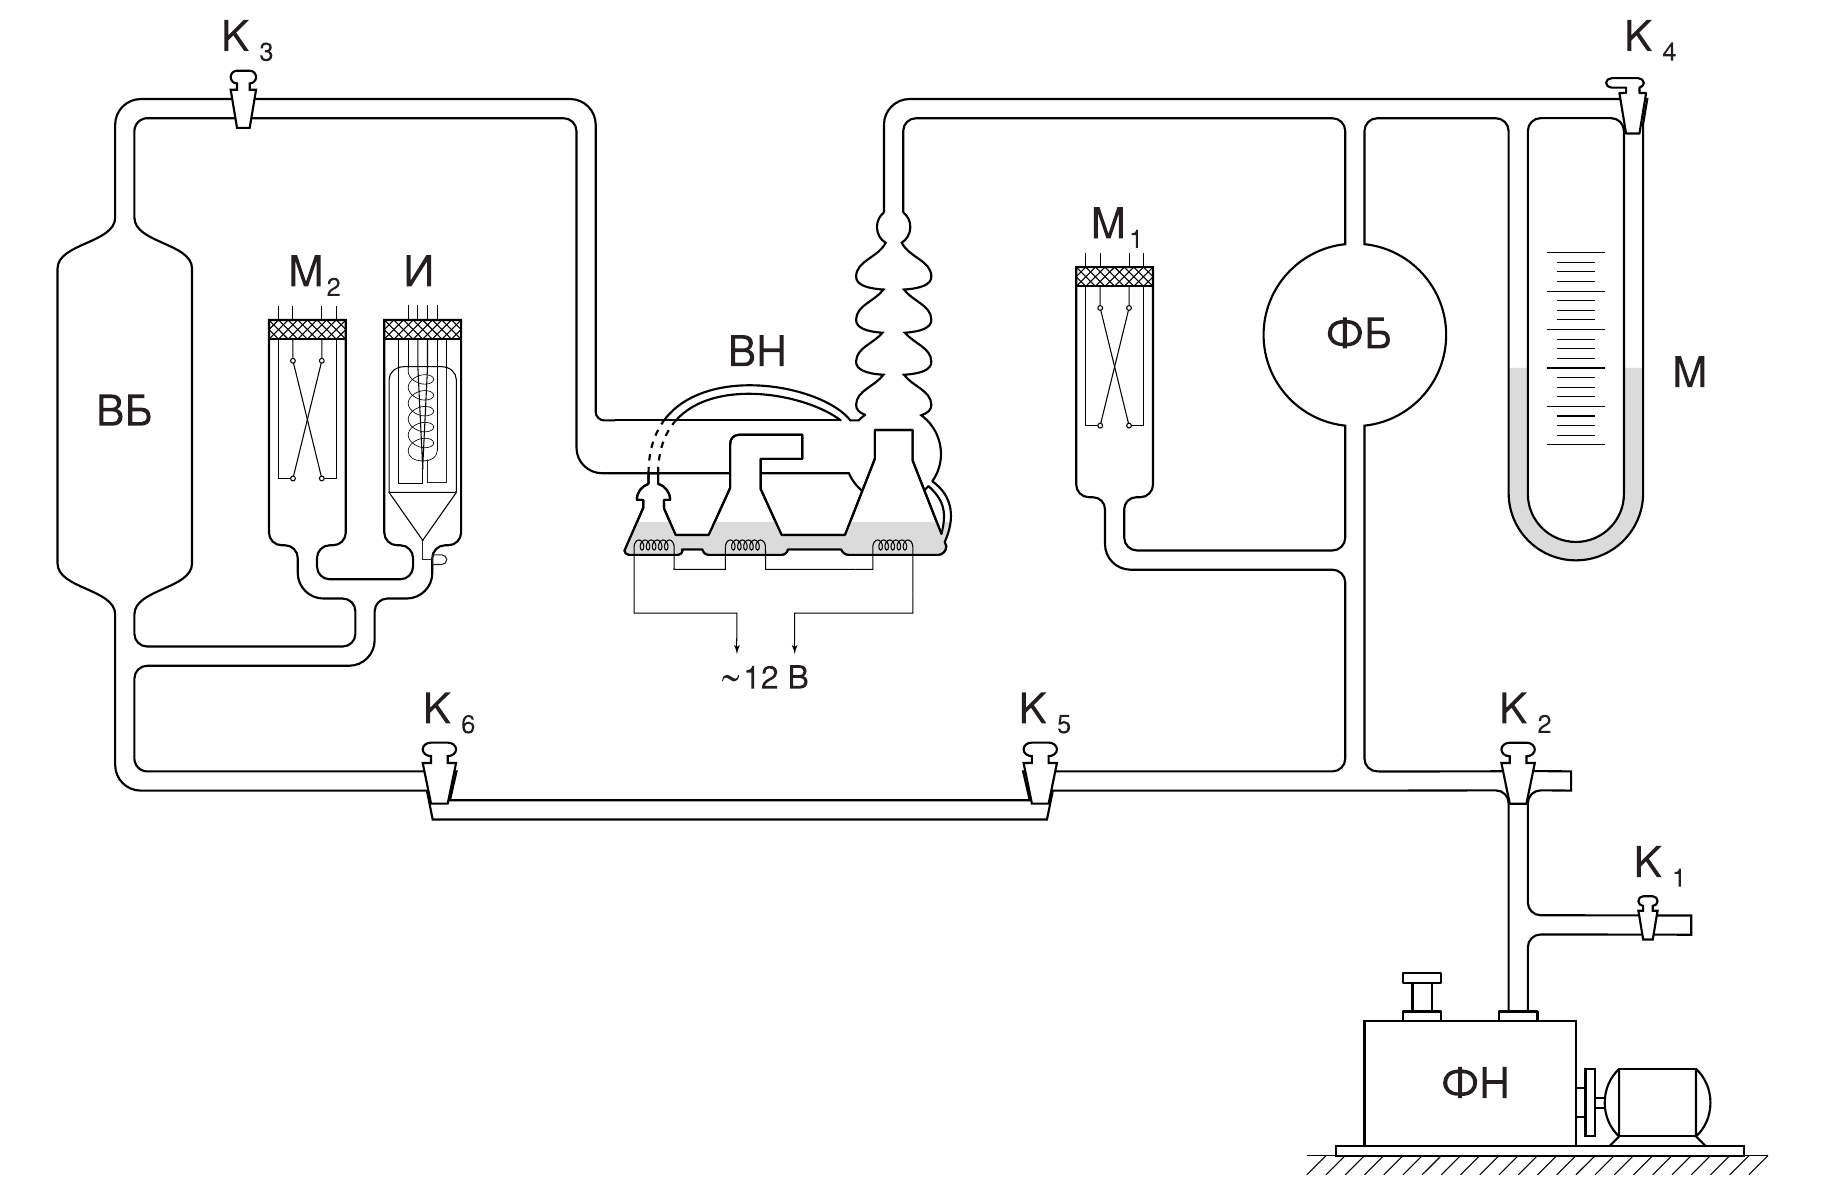
\includegraphics[width=0.9\textwidth]{data/установка.png}
  \end{center}
  \caption{Схема экспериментальной установки\label{fig:1}}
\end{figure}

Установка изготовлена из стекла и состоит из:
\begin{itemize}
  \item форвакуумного баллона (ФБ)
  \item высоковакуумного диффузионного насоса (ВН)
  \item высоковакуумного баллона (ВБ)
  \item масляного (М) и ионизационного (И) манометров
  \item термопарных манометров ($M_1$ и $M_2$)
  \item форвакуумного насоса (ФН)
  \item соединительных кранов ($K_1, \ldots, K_6$)
\end{itemize}

Все краны вакуумной установки стеклянные. Стенки кранов тонкие, пробки кранов полые и составляют одно целое с рукоятками.
Пробки кранов притерты к корпусам. Для герметизации используется вакуумная смазка.

\begin{figure} [H]
  \begin{center}
    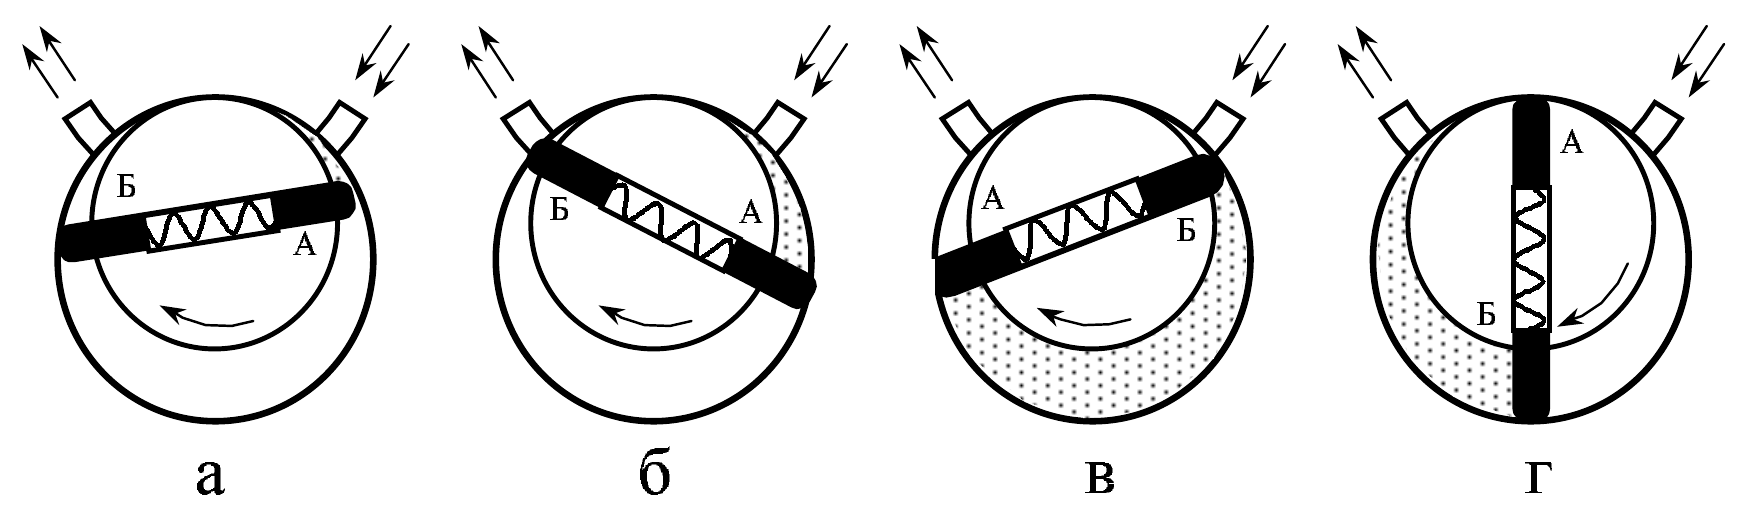
\includegraphics[width=0.9\textwidth]{data/ФН_принцип_работы.png}
  \end{center}
  \caption{Схема действия ФН.\label{fig:2}}
\end{figure}

Устройство и принцип действия \textit{форвакуумного насоса} схематически, но довольно ясно изображены на \figref{fig:2}.

\subsection{Диффузионный насос (ВН).}

\begin{figure} [H]
  \begin{center}
    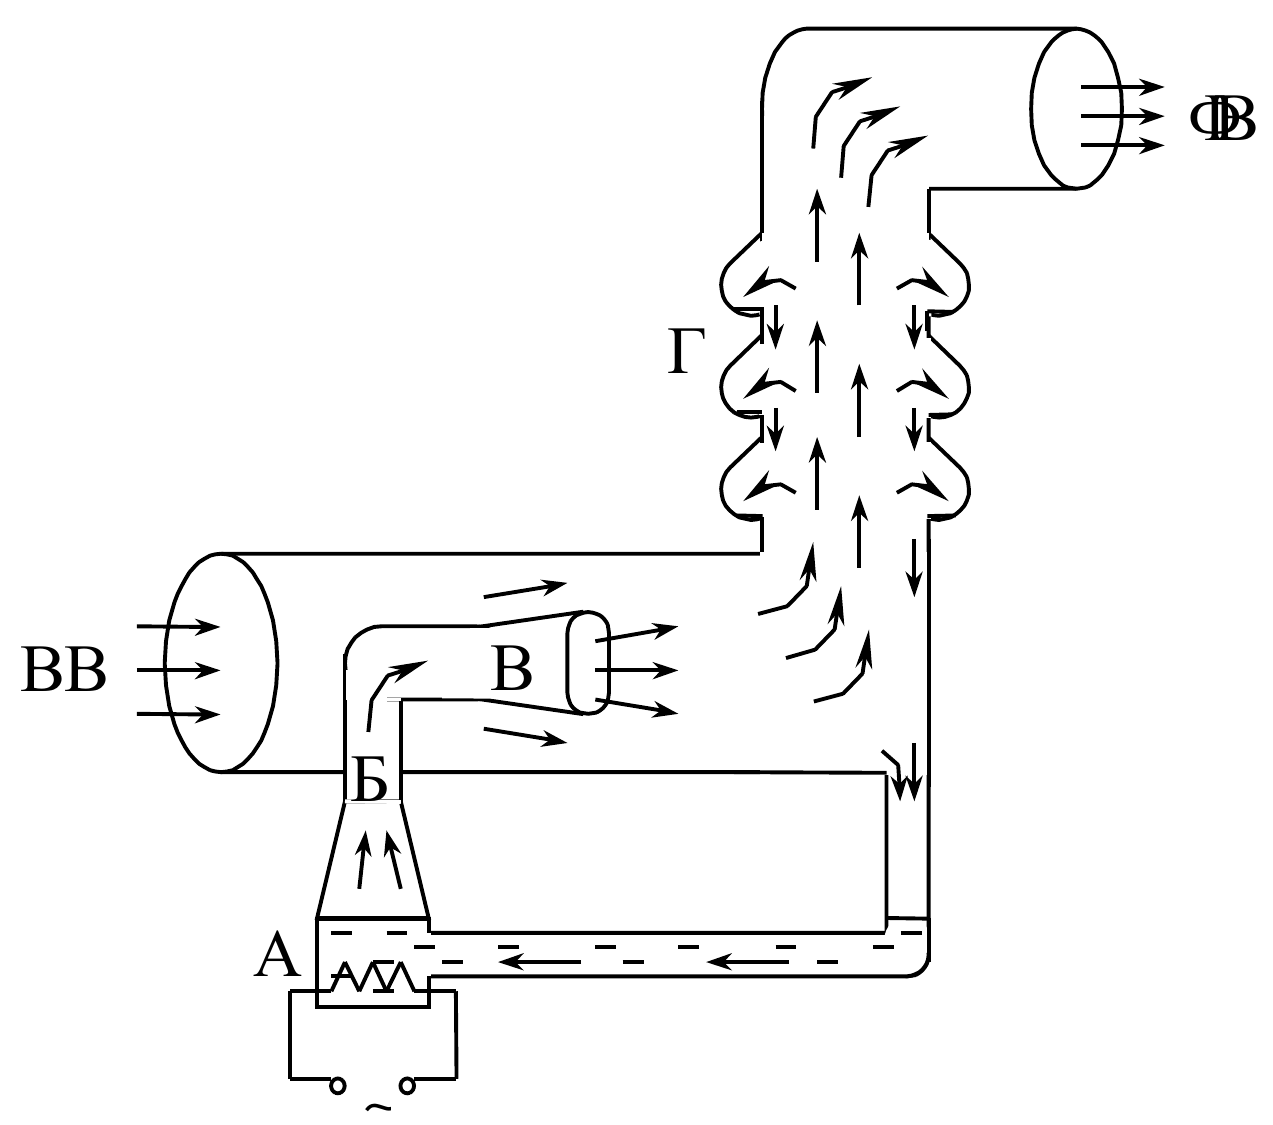
\includegraphics[width=0.7\textwidth]{data/ВН_принцип_работы.png}
  \end{center}
  \caption{Схема действия диффузионного насоса.\label{fig:3}}
\end{figure}

Масло, налитое в сосуд А, подогревается электрической печкой. Пары масла поднимаются по трубе Б и вырываются из сопла В.
Струя паров увлекает молекулы газа, которые поступают из откачиваемого сосуда через трубку ВВ.
Дальше смесь попадает в вертикальную трубу Г. Здесь масло осаждается на стенках трубы и маслосборников и стекает вниз, а оставшийся газ через трубу ФВ откачивается форвакуумным насосом.
Диффузионный насос работает наиболее эффективно при давлении, когда длина свободного пробега молекул воздуха
примерно равна ширине кольцевого зазора между соплом В и стенками трубы ВВ. В этом случае пары масла увлекают молекулы воздуха из всего сечения зазора.

Включать ВН стоит только при уже имеющемся вакууме $5 \cdot 10^{-2} \torr$.
После включения ВН, давление в системе сначала будет подниматся.
Через десять минут масло начнет испарятся, а ВН - работать.

\subsection{Масляный манометр (М).}
Две U-образные трубки, наполовину заполненные маслом.
Разница давления измеряется по разнице высот масла в двух трубках.

\begin{equation}
  \rho \approx 0.9\ \frac{\gr}{\cm^3}
  \label{val:rho}
\end{equation}
\begin{description}
  \item[$\rho$] - плотность масла в маслянном манометре.
\end{description}

\subsection{Термопарный манометр.}

% \begin{wrapfigure}{r}{50mm}
%   \begin{center}
%     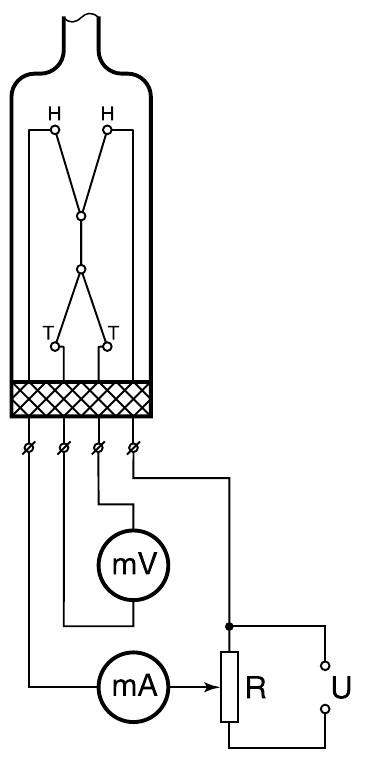
\includegraphics[width=0.9\linewidth]{data/ЛТ.png}
%     \caption{Схема термопарного манометра.\label{fig:Схема термопарного монометра}}
%   \end{center}
% \end{wrapfigure}

\seefigref{fig:Схема термопарного монометра}\\
По нити накала НН пропускается ток постоянной величины. Термопара ТТ присоединяется к милливольтметру,
показания которого определяются температурой нити накала и зависят от отдачи тепла вокружающее пространство.
Потери тепла определяются теплопроводностью нити и термопары, теплопроводностью газа, переносом тепла конвективными потоками газа внутри лампы и теплоизлучением нити (инфракрасноетепловое излучение).
В обычном режимелампы основную роль играет теплопроводность газа. При давлениях >1 торр теплопроводность газа, а вместе с ней и ЭДС термопары практически не зависят от давления газа,
и прибор не работает. При улучшении вакуума средний свободный пробег молекул становится сравнимым с диаметром нити, теплоотвод падает и температура спая возрастает. При вакууме $~10^{-3}$ торр
теплоотвод, осуществляемый газом, становится сравнимым с другими видами потерь теплаи температура
нити становится практически постоянной. \\
Градуировочная кривая термопарного манометра приведена на \seefigref{graph:M}.

\begin{figure}[H]
  \begin{minipage}{0.3\textwidth}
    \centering
    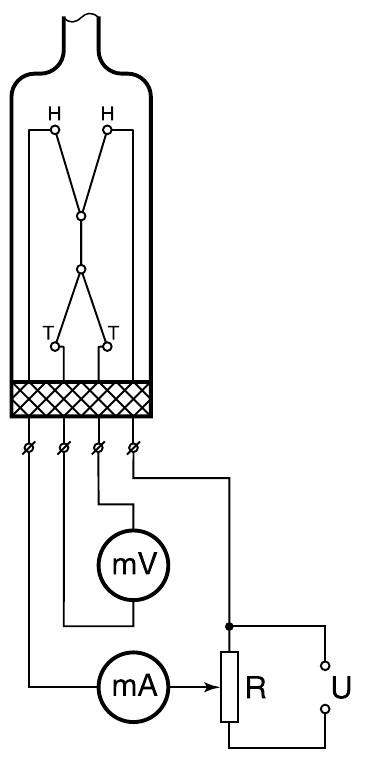
\includegraphics[width=0.9\linewidth]{data/ЛТ.png}
    \caption{Схема термопарного манометра.\label{fig:Схема термопарного монометра}}
  \end{minipage}\hfill
  \begin{minipage}{0.8\textwidth}
    \centering
    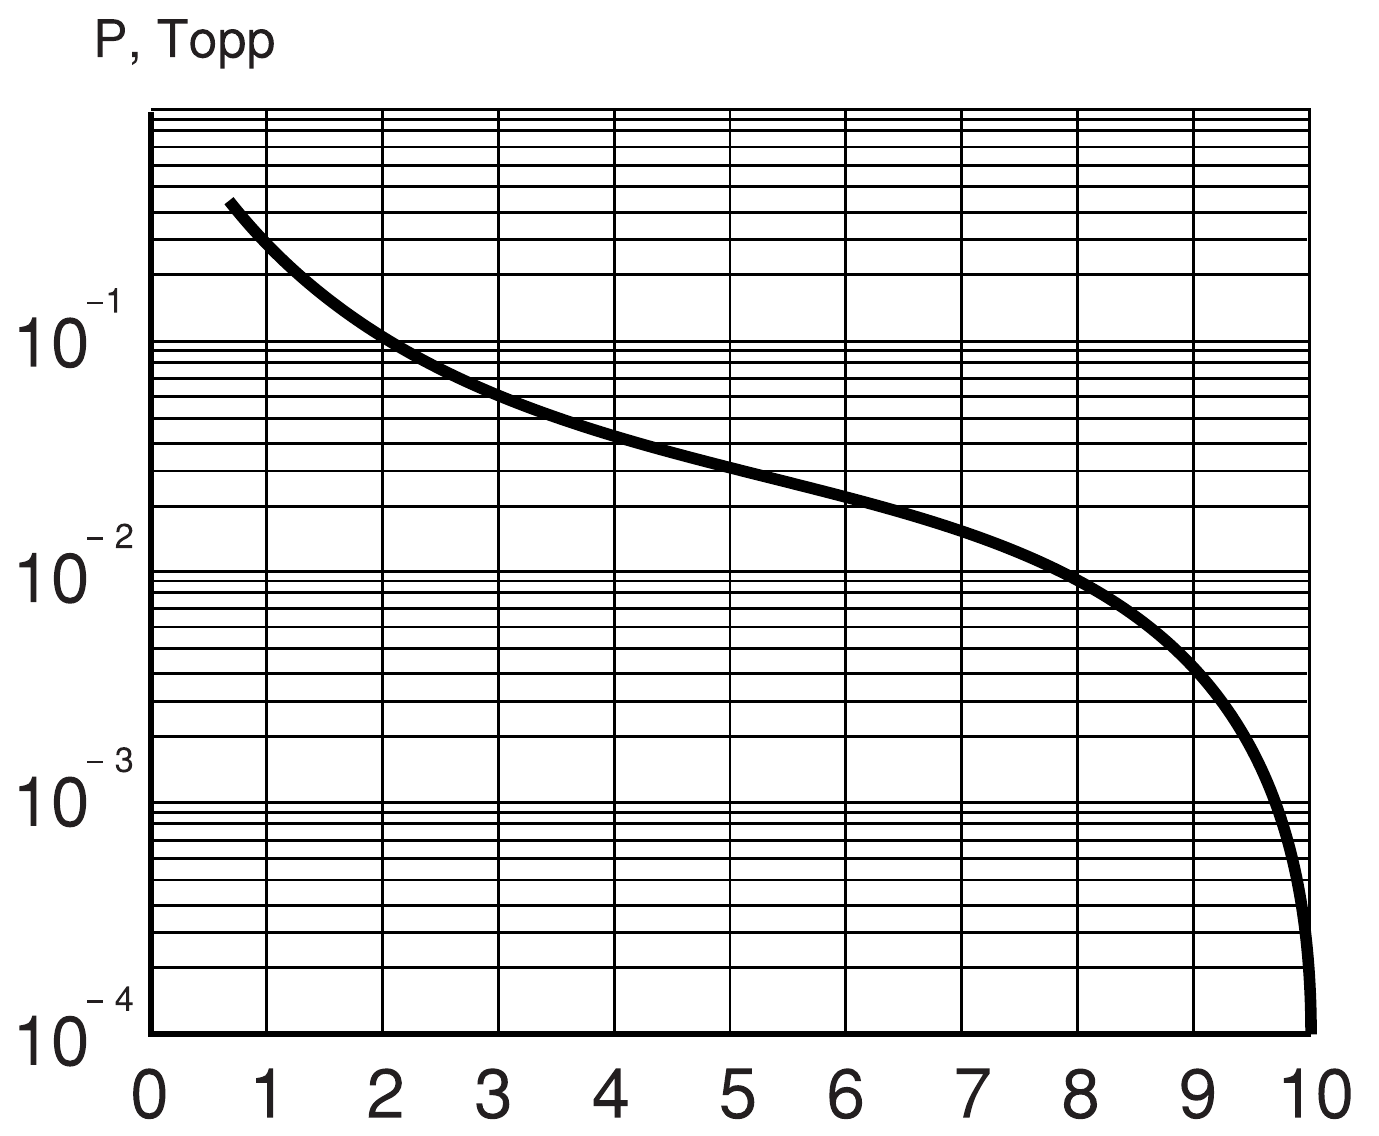
\includegraphics[width=0.8\textwidth]{data/ТМ_кривая.png}
    \caption{Градуировочная кривая термопары.\label{graph:M}}
  \end{minipage}\hfill
\end{figure}

\subsection{Ионизационный манометр.}
Схема ионизационного манометра изображена на \seefigref{fig:схема_ионизационной_лампы}.
Он представляет собой трехэлектродную лампу. Электроны испускаются накаленным катодом и увлекаются электрическим полем к аноду, имеющему вид спирали. Проскакивая за ее витки,электроны замедляются полем коллектора и возвращаются к катоду, а от него вновь увлекаются к аноду.
Прежде чем осесть на аноде, они успевают много раз пересечь пространство между катодом и коллектором.
На своем пути электроны ионизуют молекулы газа. Ионы, образовавшиеся между анодом и коллектором, притягиваются полем коллектора и определяют его ток.
Ионный ток в цепи коллектора пропорционален плотности газа и поэтому может служить мерой давления.
Вероятность ионизации зависит от рода газа, заполняющего лампу (а значит, и откачиваемый объем).
Калибровка манометра верна, если остаточным газом является воздух. Накаленный катод ионизационного манометра перегорает, если давление в системе превышает $10^{-3}$ торр.
Поэтому включать ионизационный манометр можно, только убедившись по термопарному манометру, что давление в системе не превышает $10^{-3}$ торр.
При измерении нить ионизационного манометра сильно греется. При этом она сама, окружающие ее электроды и стенки стеклянного баллона могут десорбировать поглощенные ранее газы.
Выделяющиеся газы изменяют давление в лампе и приводят к неверным показаниям. Поэтому перед измерениями ионизационный манометр прогревается (обезгаживается) в течение 10–15 мин. Для прогрева пропускается ток через спиральный анод лампы.

\begin{figure}[H]
  \centering
  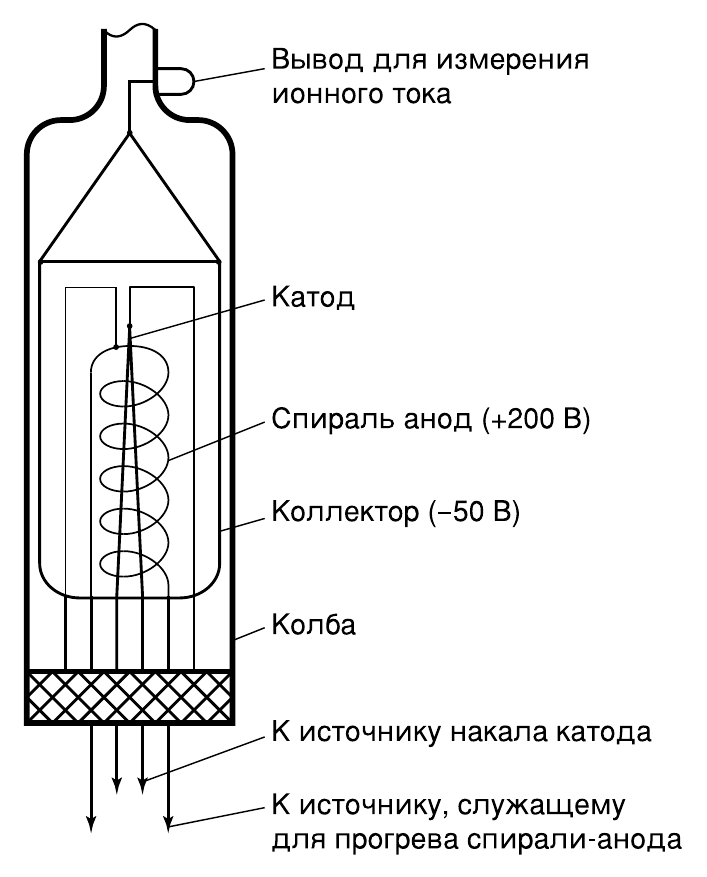
\includegraphics[width=0.5\textwidth]{6.png}
  \caption{Схема ионизационной лампы ЛМ-2.\label{fig:схема_ионизационной_лампы}}
\end{figure}

\section{Теоретическая часть}

\paragraph{Процесс откачки: }
Производительность насоса определяется скоростью откачки $W$ (л/с). Скорость откачки форвакуумного насоса равна емкости воздухозаборной камеры, умноженной на число оборотов в секунду.

Обозначим через $Q_\text{д}$ количество газа, десорбирующегося с поверхности откачиваемого объема в единицу времени,
$Q_\text{и}$ --- количество газа, проникающего в единицу времени в этот объем извне (через течи). \\
Будем считать, что насос обладает скоростью откачки $W$ и в то же время сам является источником газа. \\
Пусть $Q_\text{н}$ — поток газа, поступающего из насоса назад в откачиваемую систему. \\
Пусть $Q=Q_\text{д} + Q_\text{и} + Q_\text{н}$ (моль/с).

Получаем формулу:
\begin{equation}
  -V\d{P}=\left(P W - Q \cdot RT\right)\d{t}
\end{equation}

При предельном давлении $\d{P}=0$ и поэтому получаем:
\begin{equation}
  P_\text{пр} W = Q \cdot RT; \quad
  W = \frac{Q \cdot RT}{P_\text{пр}}
\end{equation}

Подставляя получаем
\begin{equation}
  -V\d{P}=W\left(P-P_\text{пр}\right)\d{t}
\end{equation}
Интегрируем полученное ур-е и получаем
\begin{equation}
  P-P_\text{пр}=(P_0 - P_\text{пр})\exp{\left(-\frac{W}{V}t\right)}
\end{equation}
Пренебрегая $P_\text{пр}$ относитеьно $P_0$
\begin{equation}
  P=P_0\exp\left(-\frac{W}{V}t\right)
\end{equation}
Как видим, величина $\tau=V/W$ показывает характерное время откачки системы.

Теперь попробуем понять чем обусловлена скорость откачки. Очевидно, скорость $W$ зависит от скорости откачки насоса $W_\text{н}$, но она так же зависит от трубопровода соединяюшего насос к откачиваемой части, т.к. если трубопровод не сможет обеспечить достаточное количество газа к входу насоса то, производительность упадет.

Попробуем описать систему математически. Пусть у нас есть насос со скоростью откачки $W_\text{н}$ и трубопровод с пропускной способностью $C$. Давление в откачиваемом объеме -- $P_1$.

\begin{equation}
  C(P_1 - P_2)=W_\text{н} P_2 \implies
  P_2=\frac{CP_1}{C+W_\text{н}} \Rightarrow
  WP_1=W_\text{н} 2=\frac{C W_\text{н}}{C + W_\text{н}} P_1
\end{equation}
Как видим, для результирующей скорости $W$ верно соотношение

\begin{equation}
  \frac{1}{W} = \frac{1}{W_\text{н}} + \frac{1}{C}
\end{equation}
Обобщая это выражение для последовательно соединенных труб получаем

\begin{equation}
  \frac{1}{W} = \frac{1}{W_\text{н}} + \frac{1}{C_1} + \frac{1}{C_2} + ...
  \label{resulting_speed}
\end{equation}
Заметим только что данные формулировки верны при молекулярном режиме течения, когда вязкое трение не имеет большого вклада в движение газа.

\paragraph{Течение газа через трубу:} Для количества газa, протекающего через трубу в условиях высокого вакуума или, как говорят, в кнудсеновском режиме, справедлива формула (см. формулу 3.6):

\begin{equation}
  \frac{d(PV)}{\d{t}} = \frac{4}{3}r^3 \sqrt{\frac{2\pi RT}{\mu}} \frac{P_2 - P_1}{L}
\end{equation}

где $r$ и $L$ соответственно радиус и длина трубы. Если пренебречь давлением $P_1$ у конца, обращенного к насосу, получаем формулу для пропускной способности трубы
\begin{equation}
  C_\text{тр} = \frac{dV}{\d{t}} = \frac{4}{3}\frac{r^3}{L}\sqrt{\frac{2\pi RT}{\mu}}
\end{equation}
Для пропускной способности отверстия (например в кранах) имеем формулу

\begin{equation}
  C_\text{отв}=S\frac{\bar{v}}{4}
\end{equation}

\section{Ход работы}
\subsection{Определение объемов форвакуумной и высоковакуумной частей установки}
\begin{enumerate}
  \item Проверим, что кран К4 открыт. Откроем все краны, кроме К1 и К2.
  \item Впустим в установку атмосферный воздух через краны К1 и К2.
  \item Закроем краны К5 и К6.
  В этих кранах и соединяющем их капилляре «запирается» $V_\text{зап}$ воздуха при атмосферном давлении.
  \[V_\text{зап} = 50 \cm^3\]
  \item Закроем краны К1 и К2, включим ФН и дадим ему откачать себя. Подключим установку к ФН краном К2 и откачаем установку до давления $10^{-2}$ торр.
  \item Повернув рукоятку крана К2, отсоединим установку от ФН. Оставим ФН работать.
  \item Закроем К3.
  \item Закроем К4.
  \item Откроем К5.
  \item  Зная $V_\text{зап}$ (см. п. 3) и $\D{h_{1,2}}$, найдем, пользуясь законом Бойля–Мариотта, объем $V_\text{фв}$ форвакуумной части.
  Считаем, что объем труб мал, по сравнению с $V_\text{фв}$ и $V_\text{вб}$.
  \[P_\text{атм} V_\text{зап} = P_1 V_\text{фв} = P_2 (V_\text{фв} + V_\text{вб})\]
  \[\D{h_1} = (25.3 \pm 0.1)\ \cm; \quad \D{h_2} = (16.3 \pm 0.1)\ \cm\]
  \[P = \rho g \D{h}. \quad~\ref{val:rho}\]
  \[P_1 = ()\ \Pa\]

\end{enumerate}

\subsection{Получение высокого вакуума и измерение скорости откачки}

\section{Вывод.}

\end{document}
